% Template file for a standard thesis
\documentclass[11pt]{isuthesis}
\usepackage[pdftex]{graphicx}
%\usepackage[utf8]{inputenc}
%\usepackage{float}
%\usepackage{graphicx}
%\usepackage[english]{babel}
\usepackage{amsmath}
\usepackage{float}

% Standard, old-style thesis
\usepackage{isutraditional}   \chaptertitle
\usepackage{comment}

% Old-style, thesis numbering down to subsubsection
\alternate
\usepackage{rotating}


% Bibliography without numbers or labels
\usepackage[round]{natbib}
\bibliographystyle{plainnat}


%Optional Package to add PDF bookmarks and hypertext links
\usepackage[pdftex,hypertexnames=false,linktocpage=true]{hyperref}
\hypersetup{
	colorlinks=true,
	linkcolor=blue,
	anchorcolor=blue,
	citecolor=blue,
	filecolor=blue,
	urlcolor=blue,
	bookmarksnumbered=true,
	pdfview=FitB
}

% Use import if there are .tex files called from chapter1.tex (a table for instance) 
\usepackage{import} 

% include path for figures
\graphicspath{{figures/}}

\newenvironment{thesis}{}{}
\excludecomment{thesis} % will exclude material that is only for the thesis


\begin{document}
\DeclareGraphicsExtensions{.jpg,.pdf,.mps,.png}
% Template Titlepage File
\title{Compare RNA-Seq Differential Expression Analysis Methods}

\author{Xiyuan Sun}
\mprof{Jarad Niemi}
\major{Statistics Department}

%--------- MASTER OF SCIENCE -------------
\degree{MASTER OF SCIENCE}
\level{master's}
\members{Jarad Niemi \\ Danniel Nettleton \\ Peng Liu}
%-----------------------------------------
\notice

%-------------  PhD Dissertation -------------------
% Add these additional lines for a Doctoral Dissertation
%\degree{Master of Science}
%\level{master}
\format{dissertation}
\committee{3}


%-----------CREATIVE COMPONENT ------------------------------
% Add these additional lines for a Creative Component
% - also comment out the \maketitle command
%\format{Creative Component}
%\submit{the graduate faculty}
\maketitle

% Optional thesis dedication
\chapter*{DEDICATION}

I would like to dedicate this thesis to ...


% Table of Contents, List of Tables and List of Figures
\pdfbookmark[1]{TABLE OF CONTENTS}{table}
\tableofcontents
\addtocontents{toc}{\def\protect\@chapapp{}} \cleardoublepage \phantomsection
\addcontentsline{toc}{chapter}{LIST OF TABLES}
\listoftables
\cleardoublepage \phantomsection \addcontentsline{toc}{chapter}{LIST OF FIGURES}
\listoffigures
% Comment out the next line if NOT using chaptertitle
\addtocontents{toc}{\def\protect\@chapapp{CHAPTER\ }}



\cleardoublepage \phantomsection This research was built on Niemi et al's approach \citep{niemi2015empirical}. Their research was supported by National Institute of General Medical Sciences (NIGMS) of the National Institutes of Health and joint National Science Foundation / NIGMS Mathematical Biology Program under award number R01GM109458.  
\cleardoublepage \phantomsection  \begin{abstract}

We simulated RNA-Seq count data based on parameters estimated from a maize RNA-Seq dataset \citep{paschold2012complementation}. We comperehensively compared six differential expression (DE) analysis methods (eBayes, edgeR, DESeq2, DESeq, sSeq, and EBSeq) and evaluated their performance by receiver operator characteristic (ROC) curves and areas under the curve (AUC). eBayes tends to give the best performance in terms of AUC. We observed the following patterns: (1) the difference among methods shrinks as proportion of DE genes (pDiff) increases; (2) the number of genes (nGenes) doesn't affect the methods performance in terms of AUC values; (3) all methods perform better when the number of samples increases. Supplementary materials accompanying this paper is on github at https://github.com/xiyuansun/kellycc. 

 \end{abstract}
        



\newpage
\pagenumbering{arabic}

% Introduction of the Thesis Template File
\chapter{OVERVIEW}



\section{Introduction}

Differential expression exists when the expected value of a phenotype differs from the expected phenotypic values of the other variety. Differential expression can occue if the mean phenotype of a variety is greater than the other variety's or less than the other variety's. I refer to the former as high differential expression (HDE) and the latter as low differential expression (LDE). There is differential expression (DE) if and only if either HDE or LDE holds. Ji et al. \cite{ji2014estimation} introduced an approach to assess gene expression heterosis using microarray data under the assumption that these data are continuous. They built a normal hierarchical model for microarray measurements of transcript abundance that allows borrowing of information across genes to estimate means and variances. They introduced an empirical Bayes framework that first estimates model hyperparameters, then estimates the posterior distribution for gene-specific parameters conditional on those hyperparameters, and finally computes heterosis probabilities based on integrals of regions under this posterior. Building on the work of Ji et al. with the normal data model, Niemi et al. \cite{niemi2015empirical}

The focus here is on methods for count-based differential expression (DE) amalyses. Thus, the starting point here is a count table of features-by-samples, such as those from the Paschold project \cite{paschold2012complementation}.

Considerable recent effort has been paid to the discovery of DE features, given a count table; recent comparisons have shown that no method dominates the spectrum of possible situations \cite{soneson2013comparison}\cite{rapaport2013comprehensive}. 

\section{RNA-Seq Count Data}

RNA-Seq is a next generation sequencing procedure of the entire transcriptome by which one can measure the expression of gene expression. The number of reads mapped to a given gene is considered to be the estimate of the expression level of that feature using the technology. The end product of a RNA-seq experiment is a sequence of read counts, typically represented as a matrix with rows representing genes and columns representing samples from two varieties, as in Table \ref{tab:RNA-Seq Data}. In this example, there are $V=2$ varieties, $J_1 = 2$ samples in the first variety, $J_2=2$ samples in the second variety, and $G=10000$ genes. My interest is in the detection of differentially expressed genes among the varieties. 

\begin{table}[H]
\begin{center}
    \begin{tabular}{|c|c|c|c|c|c|}
      \hline
      Gene &Variety1 Sample1 &Variety1 Sample2 &Variety2 Sample1 & Variety2 Sample2 \\
      \hline
      1 & 4 & 1 & 100 & 88 \\
      \hline
      2 & 65 & 48 & 55 & 59 \\
      \hline
      3 & 0 & 1 & 0 & 2\\
      \hline
      ... & ... & ... & ... & ...\\
      \hline
       10000 & 3 & 1 & 1 & 2\\
       \hline
    \end{tabular}
\end{center}
\caption{RNA-Seq Count Data Example}
\label{tab:RNA-Seq Data}
\end{table}

The focus of this report is to provide a comparison of the methods related to the analysis of differential expression for RNA-seq data. In this report, I review statistical methods for detecting differential expression in the RNA-seq data, including the empirical Bayesian method. I summarize the results of a simulation study. I briefly describe some existing open source R and Bioconductor software for testing differential expression for RNA-seq data. I conclude the report with a discussion section. 




\chapter{METHOD}

\section{Estimating the difference between read counts for a given gene}

To detemine whether the read count differences between different conditions for a given gene are greater than expected by chance, differential gene expression (DGE) tools must find a way to estimate that difference \citep{dundar2015introduction}.The two basic tasks of all DGE tools are: (1) Estimate the magnitude of differential expression between two or more conditions based on read counts from replicated samples, i.e., calculate the fold change of read counts, taking into account the differences in sequencing depth and variability; (2) Estimate the significance of the difference and correct for multiple testing. 

\section{Empirical Bayes identification of gene differential expression from RNA-seq read counts}

I consider an RNA sequencing (RNA-seq) experiment that involves two genetic varieties. For each variety, replicate RNA samples are isolated and assessed for quality. Complementary DNA (cDNA) libraries, consisting of short cDNA fragments derived from RNA, are constructed. Then, next generation sequencing technology is used to determine the {\tt reads}, in the cDNA libraries \citep{niemi2015empirical}. These reads are processed using bioinformatic algorithms to match the reads to genes. The results of read processing are summarized by a gene $\times$ sample matrix of counts. See Datta and Nettleton \citep{datta2014statistical} for more details on RNA-seq experiments and data from a statistical perspective, and see \citep{paschold2012complementation} for the biological background behind the use of RNA-seq to study gene expression differentiation. 

To use RNA-seq counts to identify genes displaing differential expression (DE), I built a hierarchical to borrow information across gene-variety means and across gene-specific overdispersion parameters, estimate the hyperparameters using an empirical Bayes procedure, and calculate empirical Bayes posterior probabilities for DE. 

\subsection{Hierarchical model for RNA-seq counts}

Let $Y_{gij}$ be the count for gene $g=1,2,..., G$, variety $i=1,2$, and replicate $j=1,2,3,...,n_i$.

I assume

\begin{equation}
\label{eq:1}
Y_{gij} \stackrel{ind}{\sim} NB(\exp(\mu_{gi}+\gamma_{ij}), \exp(\psi_g))
\end{equation}

The data model involves genewise overdispersion $\psi_g$ and a mean that depends on the gene-variety combination through $\mu_{gi}$ and on the sample through $\gamma_{ij}$. The $\mu_{gi}$ terms are of primary scientific interest. The $\gamma_{ij}$ terms are normalization factors that account for differencees in the thoroughness of sequencing from sample to sample. 

Following \citep{ji2014estimation}, we reparameterize the gene-variety mean structure into the genespecific average $\beta_{g1}$ and half-variety difference $\beta_{g2}$. For our differential expression study where number of varieties is 2, we let $i=1,2$ indicate the two varieties. The reparameterization is

\begin{equation}
\label{eq:2}
\beta_{g1} = \frac{\mu_{g1}+\mu_{g2}}{2}, \beta_{g2} = \frac{\mu_{g1}-\mu_{g2}}{2}
\end{equation}

We assume a hierarchical model for the gene-specific mean parameters and overdispersion parameters. Initially, we assume the variety averages, half-variety averages, and overdispersion parameters follow normal distributions

\begin{equation}
\label{eq:3}
\beta_{g1} \stackrel{ind}{\sim} N(\eta_{\beta_1}, \sigma^2_{\beta_1}), \beta_{g2} \stackrel{ind}{\sim} N(\eta_{\beta_2} , \sigma^2_{\beta_2}), \psi_g \stackrel{ind}{\sim} N(\eta_\psi, \sigma^2_\psi)
\end{equation}

\subsection{Empirical Bayes}

We categorize the parameters of the model into gene-specific parameters $\theta = (\theta_1, ..., \theta_G)$ where $\theta_g = (\beta_{g1}, \beta_{g2}, \psi_g)$, normalization factors $\gamma = (\gamma_{11}, ..., \gamma_{V n_V})$, and hyperparameters $\pi = (\eta, \sigma)$ where $\eta = (\eta_{\beta_1}, \eta_{\beta_2}, \eta_\psi)$ and $\sigma = (\sigma_{\beta_1}, \sigma_{\beta_2}, \sigma_\psi)$. We obtain estimates for the hyperparameters and then base gene-specific inference on the posterior conditional on these estimates \citep{niemi2015empirical}.

To obtain normalization factors $\hat{\gamma}$, we use the weighted trimmed mean of $M$ values (TMM). We use edgeR to obtain genewise dispersion estimates, $\hat{\psi}_g$, and the generalized linear model methods to obtain estimates for the remaining gene-specific parameters ($\hat{\beta}_{g1}, \hat{\beta}_{g2}$)\citep{robinson2010scaling}. Using $\hat{\theta}_g = (\hat{\beta}_{g1} , \hat{\beta}_{g2}, \hat{\psi}_g)$, we estimate hyperparameters for the location and scale parameters in the hierarchical model using a central method of moments approach. 

Conditional on the estimated normalization factors $\hat{\gamma}$ and hyperparameters $\hat{\pi}$, we perform a Bayesian analysis to re-estimate the gene-specific parameters and describe their uncertainty \citep{niemi2015empirical}. Equation \ref{eq:4} shows that conditional on $\hat{\gamma}$ and $\hat{\pi}$, the gene-specific parameters are independent and therefore conditional posterior inference across the genes can be parallelized. 

\begin{equation}
\label{eq:4}
\begin{split}
& p(\theta | y, \hat{\pi}, \hat{\gamma})  \propto \\ & \prod_{g=1}^{G} \left[ \prod_{i=1}^{2} \prod_{j=1}^{n_i} NB(y_{gij} ; \exp(\mu_{gi} + \hat{\gamma}_{ij}), \exp(\psi_g)) N(\beta_{g1} ; \hat{\eta}_{\beta_1}, \hat{\sigma}^2_{\beta_1}) p(\beta_{g2} ; \hat{\eta}_{\beta_2}, \hat{\sigma}_{\beta_2}) N(\psi_g ; \hat{\eta}_{\psi}, \hat{\sigma}^2_{\psi})  \right]
\end{split}
\end{equation}

To perform the conditional posterior inference on the gene-specific parameters, we use the statistical software Stan \citep{stan2014stan} executed through the RStan interface \citep{team2016rstan}. Stan implements a Hamiltonion Monte Carlo \citep{neal2011mcmc} to obtain samples from the posterior in equation \ref{eq:4}. 


We ran 4 simultaneous chains with random initial starting values for 1000 burn-in iterations followed by another 1000 iterations retaining every fourth sample for inference. We monitored convergence using the potential scale reduction factor and effective sample size (ESS) for $\phi_g, \alpha_g$ and $\psi_g$ \citep{gelman1992inference}. If the minimum ESS was less than 1000, we reran the chains wit double the iterations for both burn-in and inference. We continued this restarting and doubling until we obtained minimum ESS greater than 1000 for all parameters. 

\subsection{Gene expression differentiation}

In the maize context that motivates this work, we are interested in differential expression (DE), i.e. either low differential expression (LDE) or high differential expression (HDE), in gene expression. For a specific gene $g$, LDE occurs when expected expression in the second variety is less than the expected expression of first variety, i.e., $\mu_{g1} > \mu_{g2}$, or equivalently, $\beta_{g2}>0$, and HDE occurs when the expected expression in the second variety is greater than the expected expression of first variety, i.e., $\mu_{g1} < \mu_{g2}$, or equivalently, $\beta_{g2}<0$. We evaluate these probabilities based on empirical Bayes estimates of their posterior probabilities, e.g., 

\begin{equation}
\label{eq:5}
P(LDE_g | y, \hat{\pi}, \hat{\gamma}) = P(\beta_{g2}>0 | y, \hat{\pi}, \hat{\gamma}) \approx \frac{1}{M} \sum_{m=1}^M I(\beta_{g2} ^ {(m)}>0)
\end{equation}

where $\beta_{g2}^{(m)}$ is the $m^{th}$ MCMC sample from the empirical Bayes posterior.

HDE probability is defined as equation \ref{eq:6}

\begin{equation}
\label{eq:6}
P(HDE_g | y, \hat{\pi}, \hat{\gamma}) = P(\beta_{g2}<0 | y, \hat{\pi}, \hat{\gamma}) \approx \frac{1}{M} \sum_{m=1}^M I(\beta_{g2} ^ {(m)}<0)
\end{equation}

I construct a ranked list of genes according to the maximum of gene's LDE and HDE probabilities. Geneticists can use this list to prioritize future experiments to understand the molecular genetic mechanisms for differential expression \citep{niemi2015empirical}. 

I will use the term ebayes to refer to the approach defined in Sections 2.1 - 2.2 and we are assuming normal distribution for half-variety differences.


\section{Simulation study based on a maize experiment}

To assess the efficacy of ebayes method to identify genes demonstrating DE, I used a maize dataset with two varieties B73 and Mo17\citep{paschold2012complementation} to determine realistic parameter values for a simulation study.I compared ebayes method to approaches using the R packages {\tt sSeq, DESeq, edgeR, EBSeq, and DESeq2}.

I used ebayes method to obtain normalization factors $\hat{\gamma}$ and gene-specific parameter estimates $\hat{\theta}_g$ for all genes using the {\tt edgeR} package\citep{robinson2010edger} applied to the maize data\citep{paschold2012complementation} on $27619$ genes with average count at least one and at most two zeros read counts for each variety across all the replicates. This analysis produced sample-specific normalization factors of $\hat{\gamma} = (0.923, 0.932, 1.029, 1.022, 0.973, 0.972, 1.063, 1.098)$. The gene-specific parameter estimates were treated as the true parameter values for the simulation study so that my simulated datasets mimicked the existing structure among the gene-variety means of the original maize data.

Using these parameters and normalization factors, I simulated data according to the negative binomial model in equation \ref{eq:1} independently for each gene. For each simulation, I analyzed a subset of $nGenes=1000$ or $nGenes=10000$ selected randomly from original maize count data. I repeated the simulation 5 times for each of 2, 4, and 8 replicates per variety, each of $1\%, 10\%, 30\%$ differentiation expression proportions, reusing normalization factors. 

Given the parameters gene-specific parameter estimates $\hat{\theta}_g$, I set up the simulation scenarios as the following table \ref{tab:Scenario}:

\begin{table}[H]
\centering
\begin{tabular}{|r|r|r|r|r|}
\hline
sc & nGenes & nSamples & pDiff \\ 
\hline
1 & 10000 & 8 & 0.10 \\ 
\hline
2 & 10000 & 8 & 0.30 \\ 
\hline
3 & 10000 & 8 & 0.01 \\
\hline
4 & 10000 & 4 & 0.10 \\
\hline
5 & 10000 & 4 & 0.30 \\
\hline
6 & 10000 & 4 & 0.01 \\ 
\hline
7 & 10000 & 16 & 0.10 \\
\hline
8 & 10000 & 16 & 0.30 \\ 
\hline
9 & 10000 & 16 & 0.01 \\
\hline
10& 1000 & 8 & 0.10 \\
\hline
11 & 1000 & 8 & 0.30 \\
\hline
12 & 1000 & 8 & 0.01 \\ 
\hline
13 & 1000 & 4 & 0.10 \\
\hline
14 & 1000 & 4 & 0.30 \\
\hline
15 & 1000 & 4 & 0.01 \\ 
\hline
16 & 1000 & 16 & 0.10 \\
\hline
17 & 1000 & 16 & 0.30 \\ 
\hline
18 & 1000 & 16 & 0.01 \\ 
\hline
\end{tabular}
\caption{Simulation Scenario Table}
\label{tab:Scenario}
\end{table}



\section{Alternative DGE tools}

Among the alternative methods, {\tt sSeq}\citep{10.1093/bioinformatics/btt143}, {\tt DESeq}\citep{anders2010differential}, {\tt edgeR}\citep{robinson2007moderated}\citep{robinson2010edger}, {\tt EBSeq}\citep{leng2013ebseq}, and {\tt DESeq2}\citep{love2014moderated} assume the Negative Binomial distribution. I biefly overview these approaches. 






\section{Methods Comparison Result}

Figure \ref{auc} is my facetted auc plot.

\begin{figure}[h!tb] 
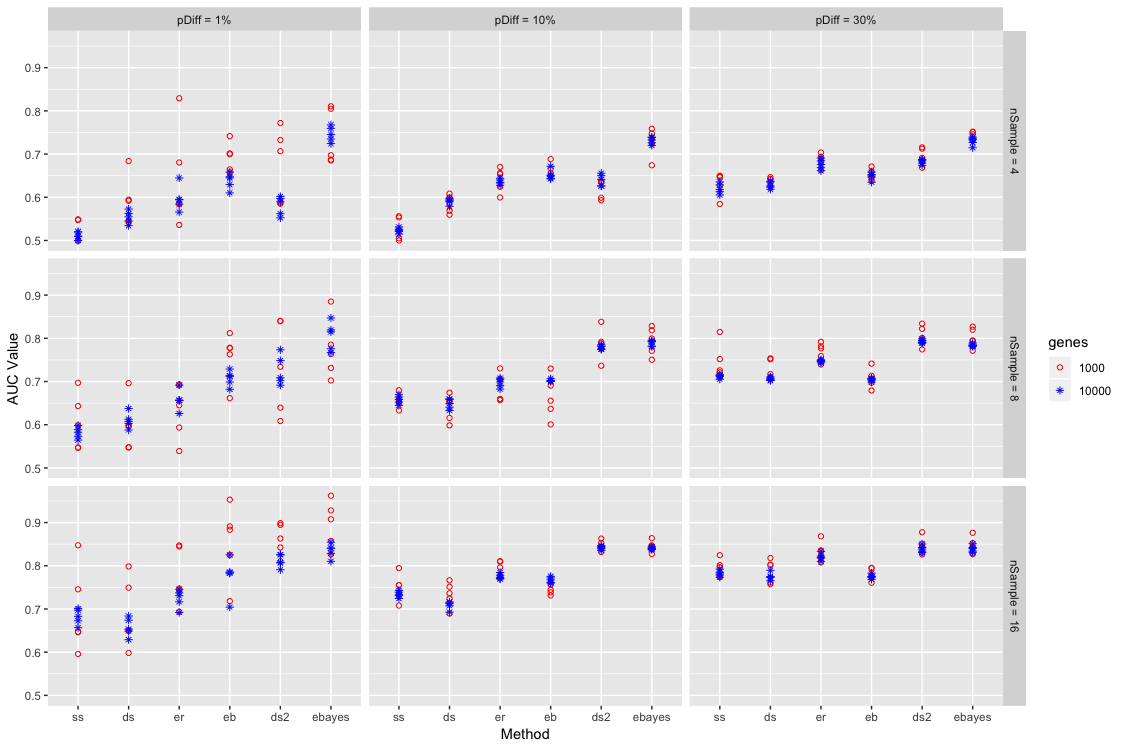
\includegraphics[scale=0.4]{auc_facet_plot}
\caption{Facet AUC Plot}
\label{auc}
\end{figure}



%\appendixtitle 
%\appendix
%\include{appendix1}
%\include{appendix2}


\renewcommand{\bibname}{\centerline{BIBLIOGRAPHY}}
\unappendixtitle
\newpage
\phantomsection
%\addcontentsline{toc}{chapter}{BIBLIOGRAPHY}
\bibliographystyle{plain}
\bibliography{mybib}

\end{document}
